\section{Presentation of the context}\label{sec:presentationOfTheContext}

\subsection{Aim of MeltyFi protocol}
The aim of MeltyFi is to define a new protocol for lending and borrowing with NFT collateral based on peer-to-pool design, solving some of the problems that plague these types of DeFi platforms.
\\
\indent MeltyFi infact is builted in different way. It is a peer-to-pool design-based lending and borrowing protocol in which the loan collateral is NFT and the funds are raised through a lottery ticket foundraising mechanism. There is no floor price dependence, so no liquidation risk. This is because the borrower creates a lottery and puts up an NFT. The lottery tickets, called WonkaBars, are sold to multiple lenders so that the borrower gets liquidity.
\\
\indent If the borrower repays the loan before the set maturity date, the NFT is returned to him or her and the lenders are repaid. If the borrower does not repay, on the maturity date the NFT is sent to the lottery winner.
\\
\indent It is also easy for the borrower to get the loan because of the peer-to-pool design, in which there are multiple lenders and not just one. MeltyFi rewards with ChocoChips (\$CHOC) borrowers who repay their loans and all lenders who melt their WonkaBars.
\\
\indent With this mechanism, as we will see, it is possible to obtain a protocol resistant to many problems and which provides benefits to all users who use it.

\subsection{The chocolate factory inside MeltyFi}
In the MeltyFi protocol, each NFT is comparable to a \textbf{chocolate bar}. When the borrower applies for a loan, they decide how many squares of chocolate to divide the bar (their NFT) and what the price is for each piece. In doing so, the chocolate bar (the NFT) is actually breaking down into small squares of chocolate (the \textbf{WonkaBars}), smaller than the bar itself. In this way, therefore, the borrower requests the loan and the illiquid and inseparable NFT is starting to lose these two properties (\textbf{it is melting}). Once this process is complete, lenders can decide whether and how many WonkaBars to buy. By buying a WonkaBar, the lender is financing the loan requested by the borrower. 
\\
\indent In the event that the borrower repays the loan, the lender can melt the purchased WonkaBars to receive back the capital employed, plus the premium for having employed this capital (the \textbf{ChocoChips}, the fragments produced by the chocolate bar when dividing into chocolate squares).
\\
\indent In the event that the borrower does not repay the loan, all WonkaBar holders compete to win the NFT collateralized by the loan because the NFT is inseparable and only one WonkaBar holder can win it. Just like in the chocolate factory \cite{chocolatefactory}, at this point the WonkaBar holders open their WonkaBars with the hope of finding the only winning ticket (the \textbf{golden ticket}) capable of authorizing them to receive the collateral NFT as a prize. At this point, the winner can melt their WonkaBars to receive the NFT as a prize, but also the ChocoChips for using their own capital in financing the loan. Those who are not winners can still melt their WonkaBars to receive only the ChocoChips.

\subsection{Use cases}
\begin{figure}[h]
    \centering
    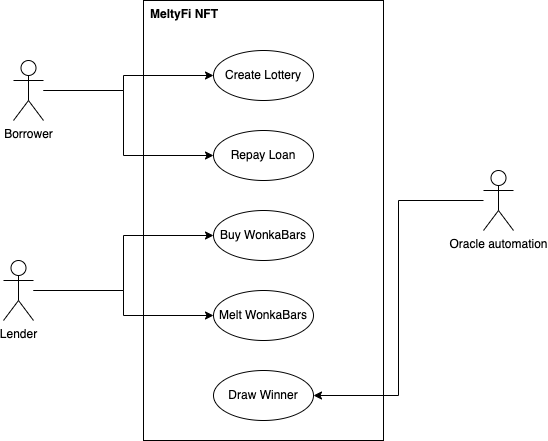
\includegraphics[width=0.8\textwidth]{figures/use_cases.png}
    \caption{Use cases of the protocol}
    \label{fig:UseCases}
\end{figure}
In \autoref{fig:UseCases} we present the use cases, five in total. There are 3 actors:
\begin{itemize}
    \item The \textbf{Lender} that can \textbf{Create Lottery} (\autoref{fig:CreateLottery}) and \textbf{Repay Loan} (\autoref{fig:RepayLoan}).
    \item The \textbf{Borrower} that can \textbf{Buy WonkaBars} (\autoref{fig:BuyWonkaBars}) and \textbf{Melt Wonkabars} (\autoref{fig:MeltWonkaBars}). 
    \item The \textbf{Oracle automation} (\autoref{fig:DrawWinner}) that can draw a winner for an expired lottery.
\end{itemize}
As follows, the only two possible scenarios that can arise within the protocol are described.

\subsubsection{Scenario 1: Borrower creates a lottery and repays the loan}
After a borrower creates a lottery, lenders can buy WonkaBars and fund the borrower. The borrower immediately receives 95\% of the price for each WonkaBar sold, while the remaining 5\% is kept by the MeltyFiDAO. After some time, but before the lottery expires, the borrower can repay the loan to cancel the lottery. They are awarded some \$CHOC and the NFT is given back to them. At this point, lenders can melt their WonkaBars and be refunded of their investment. They are also awarded with some \$CHOC.

\subsubsection{Scenario 2: Borrower creates a lottery but doesn't repay the loan}
If a borrower doesn't repay the loan before the expire date of their lottery, a winner is drawn among the lenders and the lottery is marked as concluded. Now lenders can melt their WonkaBars and still be awarded with \$CHOC, but they won't be refunded of the investment since the lottery took place. The winner lender also receives their prize NFT after melting their first WonkaBar.

\subsection{Why using a blockchain}
Blockchain provides a decentralized and distributed system for recording and tracking transactions. This means that there is no single point of failure or control, making the system more resilient and secure. Additionally, the use of cryptography and consensus algorithms ensures that transactions are immutable and tamper-proof, providing a high level of security and trust for users of the protocol, very much needed in case of lending and borrowing to people we don't know and don't trust.
\\
\indent Ethereum was the blockchain of choice.
The use of NFTs as collateral also aligns well with Ethereum, as it is currently the leading blockchain platform for NFTs. Additionally, Ethereum's large and active developer community would likely provide the necessary support for the development and maintenance of the protocol.
Another key feature of Ethereum leveraged by MeltyFi is smart contract functionality. It is seamless to think of MeltyFi as a smart contract, since it has to manage things already on blockchain. Using smart contracts it is possible to automate processes such as loan origination, collateral management, and loan repayment, reducing the need for intermediaries, and possible preferences that they could make, beside increasing efficiency.
\\
\indent In summary, the MeltyFi protocol utilizes blockchain technology to provide a secure, transparent and decentralized platform for lending and borrowing with NFTs as collateral. The decentralized nature of blockchain ensures that the platform is resilient and the smart contract functionality ensures that the process is efficient. Together, these capabilities make blockchain an essential technology for the MeltyFi protocol.

\begin{figure}[h]
    \centering
    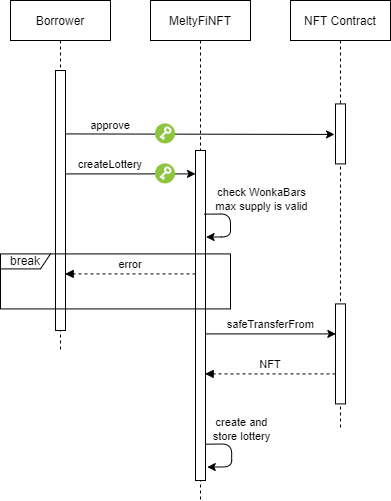
\includegraphics[width=0.8\textwidth]{figures/CreateLottery.png}
    \caption{CreateLottery sequence diagram}
    \label{fig:CreateLottery}
\end{figure}

\begin{figure}[h]
    \centering
    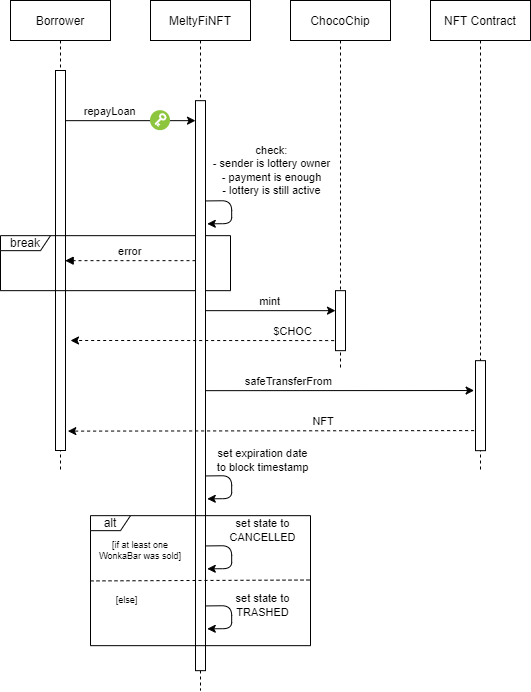
\includegraphics[width=\textwidth]{figures/RepayLoan.png}
    \caption{RepayLoan sequence diagram}
    \label{fig:RepayLoan}
\end{figure}

\begin{figure}[h]
    \centering
    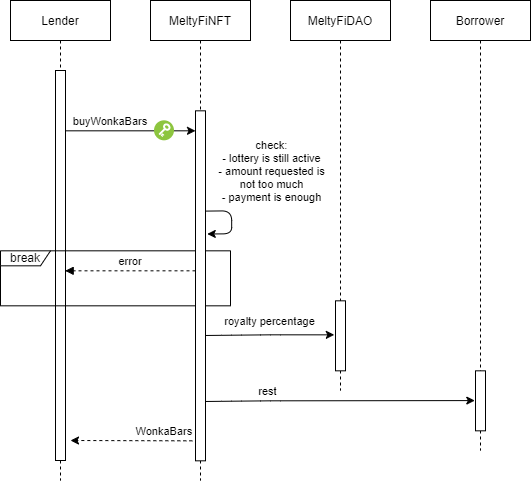
\includegraphics[width=\textwidth]{figures/BuyWonkaBars.png}
    \caption{BuyWonkaBars sequence diagram}
    \label{fig:BuyWonkaBars}
\end{figure}

\begin{figure}[h]
    \centering
    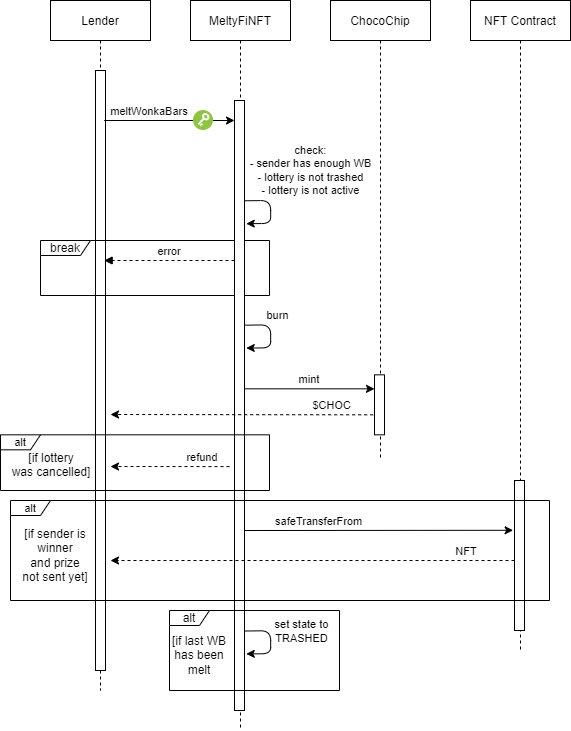
\includegraphics[width=\textwidth]{figures/MeltWonkaBars.png}
    \caption{MeltWonkaBars sequence diagram}
    \label{fig:MeltWonkaBars}
\end{figure}

\begin{figure}[h]
    \centering
    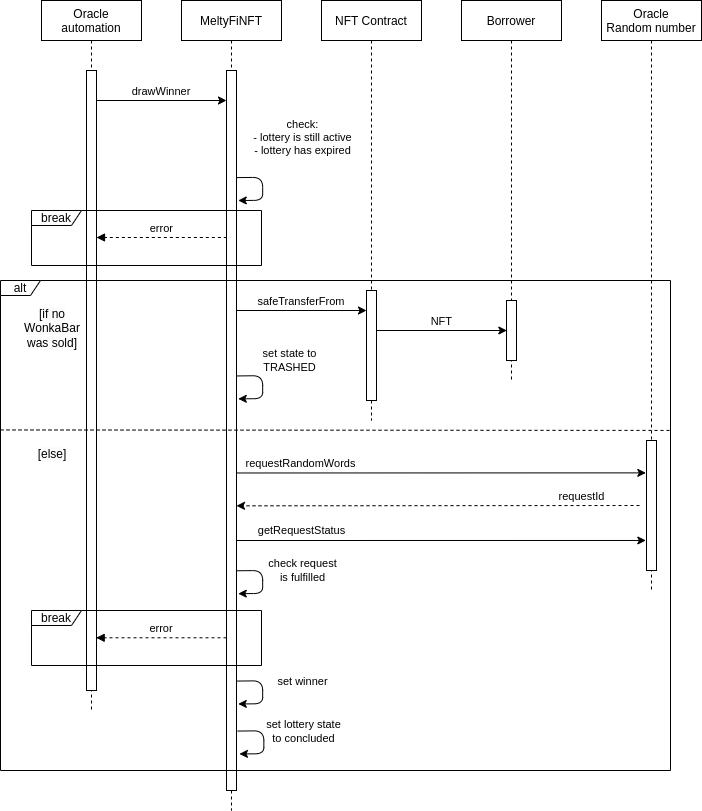
\includegraphics[width=\textwidth]{figures/DrawWinner.png}
    \caption{DrawWinner sequence diagram}
    \label{fig:DrawWinner}
\end{figure}